\documentclass[12pt]{article}

% 頁面設置
\usepackage[right=20mm, bottom=30mm, left=20mm]{geometry} % 頁面邊界
% \usepackage{multicol} % 頁面分欄
% \setlength{\columnsep}{1pt} % 欄間距
\usepackage{float} % 浮動物件 (圖表 H)

% 字體設定
\usepackage{type1cm} % 設定字體大小
\usepackage{xeCJK} % 中文字體
% \setCJKmainfont{Noto Sans TC}
\setCJKmainfont{kaiu.ttf} % 標楷體

% 套件區
\usepackage{enumitem} % 列表 (enumerate, itemize)
\usepackage{array} % 表格
\usepackage{makecell} % 表格換行
\usepackage{graphicx} % 圖片
\usepackage{longtable} % 長表格
\usepackage{indentfirst} % 自動首行縮排
\usepackage{fancyhdr} % 頁首頁尾
\usepackage{lastpage} % 最後一頁的頁數
\renewcommand{\arraystretch}{1.45} % 表格行高
\usepackage{collcell}

% 使用 hyperref 並設定
\usepackage[unicode=true,pdfusetitle,
 bookmarks=true,bookmarksnumbered=false,bookmarksopen=false,
 breaklinks=false,pdfborder={0 0 0},backref=true,colorlinks=false]
 {hyperref}

% \usepackage{amssymb} % 數學符號
% \usepackage[fleqn]{amsmath} % 數學排版, fleqn 選項讓數學式靠左對齊
% \usepackage{tikz} % 繪圖
% \usepackage{pgfplots} % 圖表
% \usepackage{caption} % 圖表標題
% \usepackage{subcaption} % 圖表子標題
% \usepackage{subfig} % 圖表子圖

% tikz 設定
% \tikzset{every state, accepting/.style={double distance=2pt}}
% \captionsetup[figure]{labelfont={bf},name={圖},labelsep=period}
% \usetikzlibrary{automata, positioning, arrows}

% fancyhdr 設定
\pagestyle{fancy}
\renewcommand{\footnotesize}{\normalsize} % 設定腳註字型大小
\renewcommand{\headrulewidth}{0pt} % 不要有頁首橫線
\renewcommand{\footrulewidth}{0pt} % 不要有頁尾橫線

\lhead{}
\chead{2023年全國大專校院智慧創新暨跨域整合創作競賽 - 作品測試文件}
\rhead{}
\lfoot{}
\cfoot{}
\rfoot{ 共 \pageref{LastPage} 頁 第 \thepage 頁} 

\begin{document}

% \makeatletter % 設定目錄字型大小
% \tableofcontents % 目錄

% 標題
% \title{}
% \author{}
% \date{}
% \maketitle

% 系統目的與範圍、提供服務與技術
\section{研究方法}

% \subsection{開發框架}

我們使用 Flutter 作為開發框架,其具備跨平台的能力以及豐富的 UI 庫,讓我們能夠同時在 Android、iOS 及 Web 平台建置系統,並方便實現各種客製化的介面效果。




\subsection{架構設計}

我們參考了 Clean architecture 與 MVVM 來設計架構,引入依賴反轉、雙向數據綁定等特性,旨在減少模組之間的依賴與增加可重用性,使得各部分能獨立開發和測試,並使得未來對系統的修改和擴展更為容易。此外,明確的架構和分層可以幫助團隊成員更快地瞭解專案結構,並減少彼此之間的工作衝突。

我們定義了兩種資料容器:

\begin{enumerate}
    \item Entity:作為系統中的主要資料容器,包含旅程、軌跡、座標點等核心資料。
    \item QueryItem:向外部資料庫(如SQL)請求數據獲得的原始結果,格式與資料表的定義相同。
\end{enumerate}

\begin{figure}[H]
    \centering
    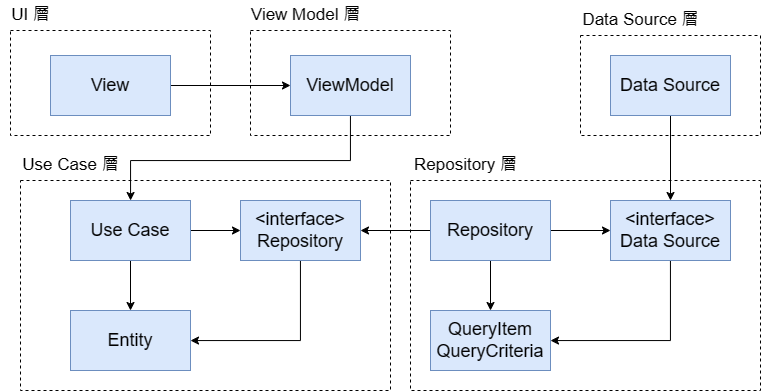
\includegraphics[width=0.8\textwidth]{assets/TT分層依賴圖.png}
    \caption{分層依賴圖}
    \label{分層依賴圖}
\end{figure}

我們將系統架構分為 Use Case、Repository、Data Source、View Model 和 UI 五層,圖~\ref{分層依賴圖} 為分層依賴圖,展示了各層內部的元件與依賴關係,以下將對各層進行詳細說明。

\begin{enumerate}

    \item Use Case 層:

    負責業務邏輯的處理,使用 Entity 作為資料容器。當 View Model 發起請求時,Use Case 會根據需求,調用 Repository 來獲得或操作數據。該層也定義了抽象的 Repository 介面。

    \item Repository 層:

    實作 Use Case 層定義的介面,負責從 Data Source 調用數據,取得 QueryItem 後轉換成 Entity 格式回傳給 Use Case。該層也定義了抽象的 Data Source 介面。

    \item Data Source 層:

    負責實際的數據存取。根據 Repository 的請求,Data Source 會去操作實際的數據來源,如資料庫、遠端服務或記憶體暫存等等,並以 QueryItem 作為回傳結果。

    \item View Model 層:

    該層為 MVVM 架構中的一部分,透過 Flutter 的 ChangeNotifier 實作。負責管理 UI 所需的狀態和邏輯。它會和 UI 進行雙向數據綁定,並透過 Use Case 處理業務邏輯和數據操作。

    \item UI 層:

    主要負責呈現使用者界面與互動。所有的 UI 元件都在這一層並組合成頁面,再透過 View Model 來獲得及顯示必要的數據。

\end{enumerate}

% \subsection{資料定義}

我們定義了幾種核心資料:

\begin{enumerate}
    \item 旅程:代表一次旅遊的所有資料,包含多個軌跡段與旅遊資料
    \item 軌跡:使用者用GPS記錄的路徑
    \item 旅遊資料:照片、影片、錄音、文字等多媒體
    \item 座標點:用一組經緯度表示一個座標點
\end{enumerate}

\subsection{AI 助手}

我們引入了 AI 助手,旨在提升使用者的旅遊體驗以及資料管理效率,能自動標記旅遊中產生的照片等資料,方便後續的查找,並讓使用者能以自然語言對話來指示 AI 執行對應動作。我們主要使用了以下技術:

\begin{itemize}
    \item AI 自動標記:利用 OpenAI CLIP 將圖片、文字記錄等多媒體資料自動標記並生成標籤。
    \item AI 對話:預定義一些基本操作,例如設定篩選條件、切換頁面、資料操作等,並利用 ChatGPT 提示工程將使用者的要求轉換成一連串操作,讓使用者能更快速完成任務。
\end{itemize}
\subsection{UI 介面設計}

為了使介面簡潔易用,我們設計了兩個主要頁面,及多個底部彈出面板(Bottom sheet),提供更高效率的操作體驗。圖~\ref{主要頁面與面板}是我們設計的主要頁面與面板。

\begin{itemize}
    \item 主要頁面:透過地圖(圖~\ref{地圖頁面})與圖庫(圖~\ref{圖庫頁面})頁面的切換,讓使用者能輕鬆查看目前的軌跡或旅遊資料,旅遊資料會根據其位置與時間順序被聚合成資料群集點,避免畫面過於雜亂。
    \item 同步資料顯示:透過主要頁面側邊的旅遊資料時間軸列表來同步兩個頁面所定位的資料群集。
    \item 快速紀錄:在地圖上方提供多功能輸入欄,能讓使用者在途中快速記錄文字筆記、拍攝照片或錄製語音。
    \item 底部彈出面板:讓使用者在不用切換頁面的情況下訪問各種功能,如獲取詳細資料(圖~\ref{旅程詳細資料面板})、與AI對話(圖~\ref{AI對話面板})、篩選資料(圖~\ref{旅遊資料篩選面板})與管理所有旅程(圖~\ref{旅程管理面板}),並能在主要頁面即時看到資料更新情況。
\end{itemize}

\newcommand{\customsubfig}[2]{
    \hspace{0.005\textwidth}
    \begin{subfigure}[t]{0.13\textwidth}
        \centering
        \includegraphics[width=\linewidth]{assets/#1.png}
        \caption{#2}
        \label{#2}
    \end{subfigure}
    \hspace{0.005\textwidth}
}

\begin{figure}[H]
    \centering
    \customsubfig{地圖頁面}{地圖頁面}
    \customsubfig{圖庫頁面}{圖庫頁面}
    \customsubfig{旅程詳細資料面板-統計資料}{旅程詳細資料面板}
    % \customsubfig{旅程詳細資料面板-軌跡列表}
    %
    % \vspace{0.5em}
    %
    % \customsubfig{AI對話面板}
    \customsubfig{AI對話面板-聊天}{AI對話面板}
    \customsubfig{旅遊資料篩選面板}{旅遊資料篩選面板}
    \customsubfig{旅程管理面板}{旅程管理面板}

    \caption{主要頁面與面板}
    \label{主要頁面與面板}
\end{figure}

\let\customsubfig\relax

% \begin{enumerate}

%     \item 地圖頁面:

%     如圖~\ref{地圖頁面},使用者可以在地圖上探索和回顧旅遊的軌跡與資料。所有的旅遊資料點將根據其地理位置與時間順序被聚合成資料群集點,以避免畫面過於複雜。側邊有一個與圖庫頁面共用的時間軸,可以同步兩個頁面要顯示的資料群集。上方的多功能輸入欄,能讓使用者在途中快速記錄文字筆記、拍攝照片或錄製語音。

%     \item 圖庫頁面:

%     如圖~\ref{圖庫頁面},以格狀排列展示所有的旅遊資料,包括圖片、筆記和語音記錄等。透過點擊側邊時間軸的資料群集,使用者能夠查看該點的所有旅遊資料。點擊旅遊資料會開啟詳細檢視視窗,並根據資料的不同類型呈現內容。

%     \item 旅程詳細資料面板:

%     如圖~\ref{旅程詳細資料面板},顯示與特定旅程相關的詳細統計資料。包括旅程的總時間、平均速度、總距離等。滑動至右側子頁面可以查看該旅程的所有軌跡資訊。

%     \item AI對話面板:

%     如圖~\ref{AI對話面板},使用者可以透過自然語言與AI助手進行對話,請求幫助或執行特定操作。例如,使用者可以請求AI助手根據地點或時間篩選旅遊資料、整理照片或提供旅程建議等。

%     \item 旅遊資料篩選面板:

%     如圖~\ref{旅遊資料篩選面板},提供一系列的篩選和排序選項,能根據標籤、地點、名稱、類別、時間等多個維度來找到和查看特定的旅遊資料。

%     \item 旅程管理面板:

%     如圖~\ref{旅程管理面板},提供一個集中的列表來管理記錄中和已完成的所有旅程。會標記目前正在記錄中的旅程,也可以選擇是否讓特定的旅程軌跡在地圖上顯示,以便於比較和回顧。

% \end{enumerate}


% 非功能性需求
\section{研究方法}

% \subsection{開發框架}

我們使用 Flutter 作為開發框架,其具備跨平台的能力以及豐富的 UI 庫,讓我們能夠同時在 Android、iOS 及 Web 平台建置系統,並方便實現各種客製化的介面效果。




\subsection{架構設計}

我們參考了 Clean architecture 與 MVVM 來設計架構,引入依賴反轉、雙向數據綁定等特性,旨在減少模組之間的依賴與增加可重用性,使得各部分能獨立開發和測試,並使得未來對系統的修改和擴展更為容易。此外,明確的架構和分層可以幫助團隊成員更快地瞭解專案結構,並減少彼此之間的工作衝突。

我們定義了兩種資料容器:

\begin{enumerate}
    \item Entity:作為系統中的主要資料容器,包含旅程、軌跡、座標點等核心資料。
    \item QueryItem:向外部資料庫(如SQL)請求數據獲得的原始結果,格式與資料表的定義相同。
\end{enumerate}

\begin{figure}[H]
    \centering
    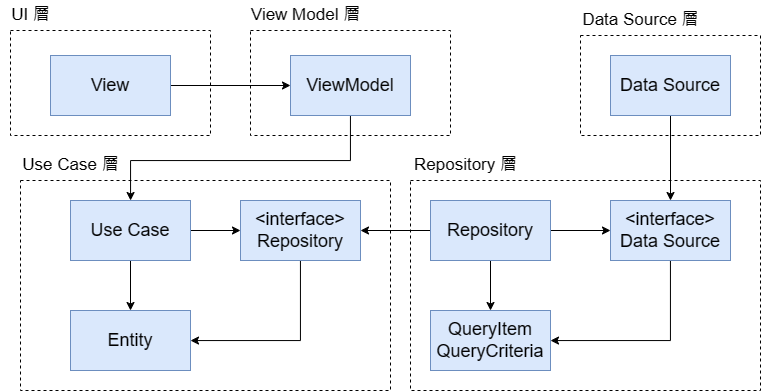
\includegraphics[width=0.8\textwidth]{assets/TT分層依賴圖.png}
    \caption{分層依賴圖}
    \label{分層依賴圖}
\end{figure}

我們將系統架構分為 Use Case、Repository、Data Source、View Model 和 UI 五層,圖~\ref{分層依賴圖} 為分層依賴圖,展示了各層內部的元件與依賴關係,以下將對各層進行詳細說明。

\begin{enumerate}

    \item Use Case 層:

    負責業務邏輯的處理,使用 Entity 作為資料容器。當 View Model 發起請求時,Use Case 會根據需求,調用 Repository 來獲得或操作數據。該層也定義了抽象的 Repository 介面。

    \item Repository 層:

    實作 Use Case 層定義的介面,負責從 Data Source 調用數據,取得 QueryItem 後轉換成 Entity 格式回傳給 Use Case。該層也定義了抽象的 Data Source 介面。

    \item Data Source 層:

    負責實際的數據存取。根據 Repository 的請求,Data Source 會去操作實際的數據來源,如資料庫、遠端服務或記憶體暫存等等,並以 QueryItem 作為回傳結果。

    \item View Model 層:

    該層為 MVVM 架構中的一部分,透過 Flutter 的 ChangeNotifier 實作。負責管理 UI 所需的狀態和邏輯。它會和 UI 進行雙向數據綁定,並透過 Use Case 處理業務邏輯和數據操作。

    \item UI 層:

    主要負責呈現使用者界面與互動。所有的 UI 元件都在這一層並組合成頁面,再透過 View Model 來獲得及顯示必要的數據。

\end{enumerate}

% \subsection{資料定義}

我們定義了幾種核心資料:

\begin{enumerate}
    \item 旅程:代表一次旅遊的所有資料,包含多個軌跡段與旅遊資料
    \item 軌跡:使用者用GPS記錄的路徑
    \item 旅遊資料:照片、影片、錄音、文字等多媒體
    \item 座標點:用一組經緯度表示一個座標點
\end{enumerate}

\subsection{AI 助手}

我們引入了 AI 助手,旨在提升使用者的旅遊體驗以及資料管理效率,能自動標記旅遊中產生的照片等資料,方便後續的查找,並讓使用者能以自然語言對話來指示 AI 執行對應動作。我們主要使用了以下技術:

\begin{itemize}
    \item AI 自動標記:利用 OpenAI CLIP 將圖片、文字記錄等多媒體資料自動標記並生成標籤。
    \item AI 對話:預定義一些基本操作,例如設定篩選條件、切換頁面、資料操作等,並利用 ChatGPT 提示工程將使用者的要求轉換成一連串操作,讓使用者能更快速完成任務。
\end{itemize}
\subsection{UI 介面設計}

為了使介面簡潔易用,我們設計了兩個主要頁面,及多個底部彈出面板(Bottom sheet),提供更高效率的操作體驗。圖~\ref{主要頁面與面板}是我們設計的主要頁面與面板。

\begin{itemize}
    \item 主要頁面:透過地圖(圖~\ref{地圖頁面})與圖庫(圖~\ref{圖庫頁面})頁面的切換,讓使用者能輕鬆查看目前的軌跡或旅遊資料,旅遊資料會根據其位置與時間順序被聚合成資料群集點,避免畫面過於雜亂。
    \item 同步資料顯示:透過主要頁面側邊的旅遊資料時間軸列表來同步兩個頁面所定位的資料群集。
    \item 快速紀錄:在地圖上方提供多功能輸入欄,能讓使用者在途中快速記錄文字筆記、拍攝照片或錄製語音。
    \item 底部彈出面板:讓使用者在不用切換頁面的情況下訪問各種功能,如獲取詳細資料(圖~\ref{旅程詳細資料面板})、與AI對話(圖~\ref{AI對話面板})、篩選資料(圖~\ref{旅遊資料篩選面板})與管理所有旅程(圖~\ref{旅程管理面板}),並能在主要頁面即時看到資料更新情況。
\end{itemize}

\newcommand{\customsubfig}[2]{
    \hspace{0.005\textwidth}
    \begin{subfigure}[t]{0.13\textwidth}
        \centering
        \includegraphics[width=\linewidth]{assets/#1.png}
        \caption{#2}
        \label{#2}
    \end{subfigure}
    \hspace{0.005\textwidth}
}

\begin{figure}[H]
    \centering
    \customsubfig{地圖頁面}{地圖頁面}
    \customsubfig{圖庫頁面}{圖庫頁面}
    \customsubfig{旅程詳細資料面板-統計資料}{旅程詳細資料面板}
    % \customsubfig{旅程詳細資料面板-軌跡列表}
    %
    % \vspace{0.5em}
    %
    % \customsubfig{AI對話面板}
    \customsubfig{AI對話面板-聊天}{AI對話面板}
    \customsubfig{旅遊資料篩選面板}{旅遊資料篩選面板}
    \customsubfig{旅程管理面板}{旅程管理面板}

    \caption{主要頁面與面板}
    \label{主要頁面與面板}
\end{figure}

\let\customsubfig\relax

% \begin{enumerate}

%     \item 地圖頁面:

%     如圖~\ref{地圖頁面},使用者可以在地圖上探索和回顧旅遊的軌跡與資料。所有的旅遊資料點將根據其地理位置與時間順序被聚合成資料群集點,以避免畫面過於複雜。側邊有一個與圖庫頁面共用的時間軸,可以同步兩個頁面要顯示的資料群集。上方的多功能輸入欄,能讓使用者在途中快速記錄文字筆記、拍攝照片或錄製語音。

%     \item 圖庫頁面:

%     如圖~\ref{圖庫頁面},以格狀排列展示所有的旅遊資料,包括圖片、筆記和語音記錄等。透過點擊側邊時間軸的資料群集,使用者能夠查看該點的所有旅遊資料。點擊旅遊資料會開啟詳細檢視視窗,並根據資料的不同類型呈現內容。

%     \item 旅程詳細資料面板:

%     如圖~\ref{旅程詳細資料面板},顯示與特定旅程相關的詳細統計資料。包括旅程的總時間、平均速度、總距離等。滑動至右側子頁面可以查看該旅程的所有軌跡資訊。

%     \item AI對話面板:

%     如圖~\ref{AI對話面板},使用者可以透過自然語言與AI助手進行對話,請求幫助或執行特定操作。例如,使用者可以請求AI助手根據地點或時間篩選旅遊資料、整理照片或提供旅程建議等。

%     \item 旅遊資料篩選面板:

%     如圖~\ref{旅遊資料篩選面板},提供一系列的篩選和排序選項,能根據標籤、地點、名稱、類別、時間等多個維度來找到和查看特定的旅遊資料。

%     \item 旅程管理面板:

%     如圖~\ref{旅程管理面板},提供一個集中的列表來管理記錄中和已完成的所有旅程。會標記目前正在記錄中的旅程,也可以選擇是否讓特定的旅程軌跡在地圖上顯示,以便於比較和回顧。

% \end{enumerate}


% 功能性需求
\section{研究方法}

% \subsection{開發框架}

我們使用 Flutter 作為開發框架,其具備跨平台的能力以及豐富的 UI 庫,讓我們能夠同時在 Android、iOS 及 Web 平台建置系統,並方便實現各種客製化的介面效果。




\subsection{架構設計}

我們參考了 Clean architecture 與 MVVM 來設計架構,引入依賴反轉、雙向數據綁定等特性,旨在減少模組之間的依賴與增加可重用性,使得各部分能獨立開發和測試,並使得未來對系統的修改和擴展更為容易。此外,明確的架構和分層可以幫助團隊成員更快地瞭解專案結構,並減少彼此之間的工作衝突。

我們定義了兩種資料容器:

\begin{enumerate}
    \item Entity:作為系統中的主要資料容器,包含旅程、軌跡、座標點等核心資料。
    \item QueryItem:向外部資料庫(如SQL)請求數據獲得的原始結果,格式與資料表的定義相同。
\end{enumerate}

\begin{figure}[H]
    \centering
    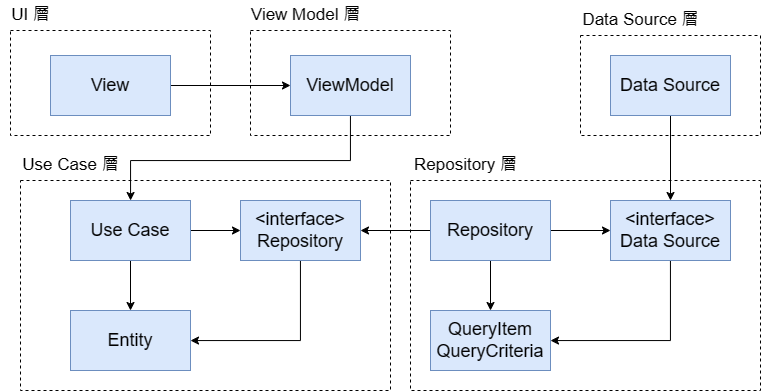
\includegraphics[width=0.8\textwidth]{assets/TT分層依賴圖.png}
    \caption{分層依賴圖}
    \label{分層依賴圖}
\end{figure}

我們將系統架構分為 Use Case、Repository、Data Source、View Model 和 UI 五層,圖~\ref{分層依賴圖} 為分層依賴圖,展示了各層內部的元件與依賴關係,以下將對各層進行詳細說明。

\begin{enumerate}

    \item Use Case 層:

    負責業務邏輯的處理,使用 Entity 作為資料容器。當 View Model 發起請求時,Use Case 會根據需求,調用 Repository 來獲得或操作數據。該層也定義了抽象的 Repository 介面。

    \item Repository 層:

    實作 Use Case 層定義的介面,負責從 Data Source 調用數據,取得 QueryItem 後轉換成 Entity 格式回傳給 Use Case。該層也定義了抽象的 Data Source 介面。

    \item Data Source 層:

    負責實際的數據存取。根據 Repository 的請求,Data Source 會去操作實際的數據來源,如資料庫、遠端服務或記憶體暫存等等,並以 QueryItem 作為回傳結果。

    \item View Model 層:

    該層為 MVVM 架構中的一部分,透過 Flutter 的 ChangeNotifier 實作。負責管理 UI 所需的狀態和邏輯。它會和 UI 進行雙向數據綁定,並透過 Use Case 處理業務邏輯和數據操作。

    \item UI 層:

    主要負責呈現使用者界面與互動。所有的 UI 元件都在這一層並組合成頁面,再透過 View Model 來獲得及顯示必要的數據。

\end{enumerate}

% \subsection{資料定義}

我們定義了幾種核心資料:

\begin{enumerate}
    \item 旅程:代表一次旅遊的所有資料,包含多個軌跡段與旅遊資料
    \item 軌跡:使用者用GPS記錄的路徑
    \item 旅遊資料:照片、影片、錄音、文字等多媒體
    \item 座標點:用一組經緯度表示一個座標點
\end{enumerate}

\subsection{AI 助手}

我們引入了 AI 助手,旨在提升使用者的旅遊體驗以及資料管理效率,能自動標記旅遊中產生的照片等資料,方便後續的查找,並讓使用者能以自然語言對話來指示 AI 執行對應動作。我們主要使用了以下技術:

\begin{itemize}
    \item AI 自動標記:利用 OpenAI CLIP 將圖片、文字記錄等多媒體資料自動標記並生成標籤。
    \item AI 對話:預定義一些基本操作,例如設定篩選條件、切換頁面、資料操作等,並利用 ChatGPT 提示工程將使用者的要求轉換成一連串操作,讓使用者能更快速完成任務。
\end{itemize}
\subsection{UI 介面設計}

為了使介面簡潔易用,我們設計了兩個主要頁面,及多個底部彈出面板(Bottom sheet),提供更高效率的操作體驗。圖~\ref{主要頁面與面板}是我們設計的主要頁面與面板。

\begin{itemize}
    \item 主要頁面:透過地圖(圖~\ref{地圖頁面})與圖庫(圖~\ref{圖庫頁面})頁面的切換,讓使用者能輕鬆查看目前的軌跡或旅遊資料,旅遊資料會根據其位置與時間順序被聚合成資料群集點,避免畫面過於雜亂。
    \item 同步資料顯示:透過主要頁面側邊的旅遊資料時間軸列表來同步兩個頁面所定位的資料群集。
    \item 快速紀錄:在地圖上方提供多功能輸入欄,能讓使用者在途中快速記錄文字筆記、拍攝照片或錄製語音。
    \item 底部彈出面板:讓使用者在不用切換頁面的情況下訪問各種功能,如獲取詳細資料(圖~\ref{旅程詳細資料面板})、與AI對話(圖~\ref{AI對話面板})、篩選資料(圖~\ref{旅遊資料篩選面板})與管理所有旅程(圖~\ref{旅程管理面板}),並能在主要頁面即時看到資料更新情況。
\end{itemize}

\newcommand{\customsubfig}[2]{
    \hspace{0.005\textwidth}
    \begin{subfigure}[t]{0.13\textwidth}
        \centering
        \includegraphics[width=\linewidth]{assets/#1.png}
        \caption{#2}
        \label{#2}
    \end{subfigure}
    \hspace{0.005\textwidth}
}

\begin{figure}[H]
    \centering
    \customsubfig{地圖頁面}{地圖頁面}
    \customsubfig{圖庫頁面}{圖庫頁面}
    \customsubfig{旅程詳細資料面板-統計資料}{旅程詳細資料面板}
    % \customsubfig{旅程詳細資料面板-軌跡列表}
    %
    % \vspace{0.5em}
    %
    % \customsubfig{AI對話面板}
    \customsubfig{AI對話面板-聊天}{AI對話面板}
    \customsubfig{旅遊資料篩選面板}{旅遊資料篩選面板}
    \customsubfig{旅程管理面板}{旅程管理面板}

    \caption{主要頁面與面板}
    \label{主要頁面與面板}
\end{figure}

\let\customsubfig\relax

% \begin{enumerate}

%     \item 地圖頁面:

%     如圖~\ref{地圖頁面},使用者可以在地圖上探索和回顧旅遊的軌跡與資料。所有的旅遊資料點將根據其地理位置與時間順序被聚合成資料群集點,以避免畫面過於複雜。側邊有一個與圖庫頁面共用的時間軸,可以同步兩個頁面要顯示的資料群集。上方的多功能輸入欄,能讓使用者在途中快速記錄文字筆記、拍攝照片或錄製語音。

%     \item 圖庫頁面:

%     如圖~\ref{圖庫頁面},以格狀排列展示所有的旅遊資料,包括圖片、筆記和語音記錄等。透過點擊側邊時間軸的資料群集,使用者能夠查看該點的所有旅遊資料。點擊旅遊資料會開啟詳細檢視視窗,並根據資料的不同類型呈現內容。

%     \item 旅程詳細資料面板:

%     如圖~\ref{旅程詳細資料面板},顯示與特定旅程相關的詳細統計資料。包括旅程的總時間、平均速度、總距離等。滑動至右側子頁面可以查看該旅程的所有軌跡資訊。

%     \item AI對話面板:

%     如圖~\ref{AI對話面板},使用者可以透過自然語言與AI助手進行對話,請求幫助或執行特定操作。例如,使用者可以請求AI助手根據地點或時間篩選旅遊資料、整理照片或提供旅程建議等。

%     \item 旅遊資料篩選面板:

%     如圖~\ref{旅遊資料篩選面板},提供一系列的篩選和排序選項,能根據標籤、地點、名稱、類別、時間等多個維度來找到和查看特定的旅遊資料。

%     \item 旅程管理面板:

%     如圖~\ref{旅程管理面板},提供一個集中的列表來管理記錄中和已完成的所有旅程。會標記目前正在記錄中的旅程,也可以選擇是否讓特定的旅程軌跡在地圖上顯示,以便於比較和回顧。

% \end{enumerate}


% 使用案例
\section{研究方法}

% \subsection{開發框架}

我們使用 Flutter 作為開發框架,其具備跨平台的能力以及豐富的 UI 庫,讓我們能夠同時在 Android、iOS 及 Web 平台建置系統,並方便實現各種客製化的介面效果。




\subsection{架構設計}

我們參考了 Clean architecture 與 MVVM 來設計架構,引入依賴反轉、雙向數據綁定等特性,旨在減少模組之間的依賴與增加可重用性,使得各部分能獨立開發和測試,並使得未來對系統的修改和擴展更為容易。此外,明確的架構和分層可以幫助團隊成員更快地瞭解專案結構,並減少彼此之間的工作衝突。

我們定義了兩種資料容器:

\begin{enumerate}
    \item Entity:作為系統中的主要資料容器,包含旅程、軌跡、座標點等核心資料。
    \item QueryItem:向外部資料庫(如SQL)請求數據獲得的原始結果,格式與資料表的定義相同。
\end{enumerate}

\begin{figure}[H]
    \centering
    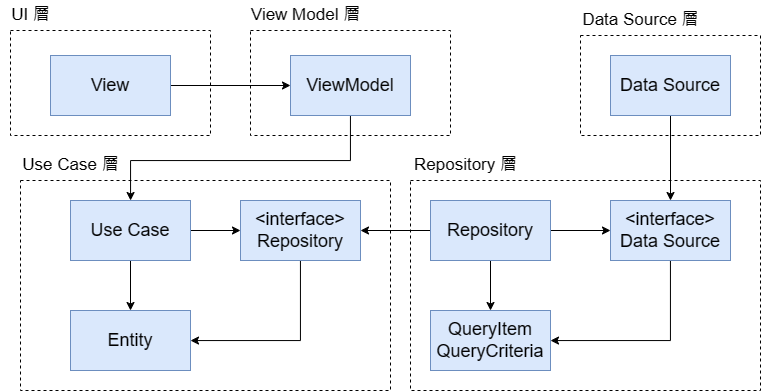
\includegraphics[width=0.8\textwidth]{assets/TT分層依賴圖.png}
    \caption{分層依賴圖}
    \label{分層依賴圖}
\end{figure}

我們將系統架構分為 Use Case、Repository、Data Source、View Model 和 UI 五層,圖~\ref{分層依賴圖} 為分層依賴圖,展示了各層內部的元件與依賴關係,以下將對各層進行詳細說明。

\begin{enumerate}

    \item Use Case 層:

    負責業務邏輯的處理,使用 Entity 作為資料容器。當 View Model 發起請求時,Use Case 會根據需求,調用 Repository 來獲得或操作數據。該層也定義了抽象的 Repository 介面。

    \item Repository 層:

    實作 Use Case 層定義的介面,負責從 Data Source 調用數據,取得 QueryItem 後轉換成 Entity 格式回傳給 Use Case。該層也定義了抽象的 Data Source 介面。

    \item Data Source 層:

    負責實際的數據存取。根據 Repository 的請求,Data Source 會去操作實際的數據來源,如資料庫、遠端服務或記憶體暫存等等,並以 QueryItem 作為回傳結果。

    \item View Model 層:

    該層為 MVVM 架構中的一部分,透過 Flutter 的 ChangeNotifier 實作。負責管理 UI 所需的狀態和邏輯。它會和 UI 進行雙向數據綁定,並透過 Use Case 處理業務邏輯和數據操作。

    \item UI 層:

    主要負責呈現使用者界面與互動。所有的 UI 元件都在這一層並組合成頁面,再透過 View Model 來獲得及顯示必要的數據。

\end{enumerate}

% \subsection{資料定義}

我們定義了幾種核心資料:

\begin{enumerate}
    \item 旅程:代表一次旅遊的所有資料,包含多個軌跡段與旅遊資料
    \item 軌跡:使用者用GPS記錄的路徑
    \item 旅遊資料:照片、影片、錄音、文字等多媒體
    \item 座標點:用一組經緯度表示一個座標點
\end{enumerate}

\subsection{AI 助手}

我們引入了 AI 助手,旨在提升使用者的旅遊體驗以及資料管理效率,能自動標記旅遊中產生的照片等資料,方便後續的查找,並讓使用者能以自然語言對話來指示 AI 執行對應動作。我們主要使用了以下技術:

\begin{itemize}
    \item AI 自動標記:利用 OpenAI CLIP 將圖片、文字記錄等多媒體資料自動標記並生成標籤。
    \item AI 對話:預定義一些基本操作,例如設定篩選條件、切換頁面、資料操作等,並利用 ChatGPT 提示工程將使用者的要求轉換成一連串操作,讓使用者能更快速完成任務。
\end{itemize}
\subsection{UI 介面設計}

為了使介面簡潔易用,我們設計了兩個主要頁面,及多個底部彈出面板(Bottom sheet),提供更高效率的操作體驗。圖~\ref{主要頁面與面板}是我們設計的主要頁面與面板。

\begin{itemize}
    \item 主要頁面:透過地圖(圖~\ref{地圖頁面})與圖庫(圖~\ref{圖庫頁面})頁面的切換,讓使用者能輕鬆查看目前的軌跡或旅遊資料,旅遊資料會根據其位置與時間順序被聚合成資料群集點,避免畫面過於雜亂。
    \item 同步資料顯示:透過主要頁面側邊的旅遊資料時間軸列表來同步兩個頁面所定位的資料群集。
    \item 快速紀錄:在地圖上方提供多功能輸入欄,能讓使用者在途中快速記錄文字筆記、拍攝照片或錄製語音。
    \item 底部彈出面板:讓使用者在不用切換頁面的情況下訪問各種功能,如獲取詳細資料(圖~\ref{旅程詳細資料面板})、與AI對話(圖~\ref{AI對話面板})、篩選資料(圖~\ref{旅遊資料篩選面板})與管理所有旅程(圖~\ref{旅程管理面板}),並能在主要頁面即時看到資料更新情況。
\end{itemize}

\newcommand{\customsubfig}[2]{
    \hspace{0.005\textwidth}
    \begin{subfigure}[t]{0.13\textwidth}
        \centering
        \includegraphics[width=\linewidth]{assets/#1.png}
        \caption{#2}
        \label{#2}
    \end{subfigure}
    \hspace{0.005\textwidth}
}

\begin{figure}[H]
    \centering
    \customsubfig{地圖頁面}{地圖頁面}
    \customsubfig{圖庫頁面}{圖庫頁面}
    \customsubfig{旅程詳細資料面板-統計資料}{旅程詳細資料面板}
    % \customsubfig{旅程詳細資料面板-軌跡列表}
    %
    % \vspace{0.5em}
    %
    % \customsubfig{AI對話面板}
    \customsubfig{AI對話面板-聊天}{AI對話面板}
    \customsubfig{旅遊資料篩選面板}{旅遊資料篩選面板}
    \customsubfig{旅程管理面板}{旅程管理面板}

    \caption{主要頁面與面板}
    \label{主要頁面與面板}
\end{figure}

\let\customsubfig\relax

% \begin{enumerate}

%     \item 地圖頁面:

%     如圖~\ref{地圖頁面},使用者可以在地圖上探索和回顧旅遊的軌跡與資料。所有的旅遊資料點將根據其地理位置與時間順序被聚合成資料群集點,以避免畫面過於複雜。側邊有一個與圖庫頁面共用的時間軸,可以同步兩個頁面要顯示的資料群集。上方的多功能輸入欄,能讓使用者在途中快速記錄文字筆記、拍攝照片或錄製語音。

%     \item 圖庫頁面:

%     如圖~\ref{圖庫頁面},以格狀排列展示所有的旅遊資料,包括圖片、筆記和語音記錄等。透過點擊側邊時間軸的資料群集,使用者能夠查看該點的所有旅遊資料。點擊旅遊資料會開啟詳細檢視視窗,並根據資料的不同類型呈現內容。

%     \item 旅程詳細資料面板:

%     如圖~\ref{旅程詳細資料面板},顯示與特定旅程相關的詳細統計資料。包括旅程的總時間、平均速度、總距離等。滑動至右側子頁面可以查看該旅程的所有軌跡資訊。

%     \item AI對話面板:

%     如圖~\ref{AI對話面板},使用者可以透過自然語言與AI助手進行對話,請求幫助或執行特定操作。例如,使用者可以請求AI助手根據地點或時間篩選旅遊資料、整理照片或提供旅程建議等。

%     \item 旅遊資料篩選面板:

%     如圖~\ref{旅遊資料篩選面板},提供一系列的篩選和排序選項,能根據標籤、地點、名稱、類別、時間等多個維度來找到和查看特定的旅遊資料。

%     \item 旅程管理面板:

%     如圖~\ref{旅程管理面板},提供一個集中的列表來管理記錄中和已完成的所有旅程。會標記目前正在記錄中的旅程,也可以選擇是否讓特定的旅程軌跡在地圖上顯示,以便於比較和回顧。

% \end{enumerate}


% 系統架構設計

% 系統介面設計

% 軟體或硬體架構設計

% 軟體或硬體模組設計

% 軟體或硬體開發環境

% 系統測試案例設計

% 系統測試報告

\end{document}